\documentclass[a4paper,12pt]{report}

\usepackage{alltt, fancyvrb, url}
\usepackage{graphicx}
\usepackage{subfigure}
\usepackage{wrapfig}
\usepackage{algorithmic}
\usepackage[utf8]{inputenc}
\usepackage{fontenc}
\usepackage{amsmath,stmaryrd,mathtools,algorithm}
\usepackage{amssymb}
\usepackage{float}
\usepackage{hyperref}
\usepackage{titlesec}

% Remove option to use English naming
\usepackage[italian]{cleveref}

% Questo commentalo se vuoi scrivere in inglese.
\usepackage[italian]{babel}

\title{Relazione per\\``DPG - Dope Party Game''}

\author{Davide Freddi\\Davide Picchiotti\\Miriana Ascenzo\\Riccardo Squarcialupi}
\date{\today}

\begin{document}
 
\maketitle

\tableofcontents

\chapter{Analisi}
\section{Requisiti}
Il software DPG - Dope Party Game consiste in un gioco a turni, in cui l'obiettivo è far arrivare il proprio personaggio in fondo a un tabellone, costituito da uno o più percorsi formati da caselle.
%
Alla fine di ogni turno, vengono fatti fare dei minigiochi a ogni giocatore.

\subsubsection{Requisiti funzionali}
\begin{itemize}
	\item il software deve presentare un menu principale all'avvio, che permetta di avviare il gioco con diverse opzioni, quali numero di giocatori e numero di CPU
	\item il gioco viene giocato da più giocatori nello stesso computer, prendendo il controllo durante il proprio turno
	\item ai giocatori viene fatto tirare un dado, che determina quanti passi vengono fatti all'interno del tabellone
	\item esistono diversi tipi di celle, che possono causare diversi eventi quando un personaggio ci finisce sopra
	\item alla fine di ogni turno viene scelto casualmente un minigioco da far fare a tutti i giocatori, e in base alla posizione nella classifica dei punteggi vengono assegnati dadi migliori o peggiori
	\item ogni CPU ha una difficoltà, che determina i suoi punteggi nei minigiochi
	\item i minigiochi possibili sono:
	\begin{itemize}
	    \item ballgame - bisogna far arrivare una palla in fondo a un percorso il prima possibile, e alcuni muri fanno tornare all'inizio se colpiti
	    \item punchygame - bisogna colpire piu' sacchi possibili, mirando nella direzione giusta
	    \item molegame - bisogna colpire più talpe possibili entro lo scadere del tempo
	    \item jumpgame - bisogna arrivare più in alto possibile rimbalzando su delle piattaforme
	\end{itemize}
\end{itemize}

\section{Analisi e modello del dominio}

Il programma partirà da un menu, che al momento opportuno avvierà il gioco.
%
All'avvio del gioco il menu notificherà il ciclo di gioco (GameCycle), che gestirà una serie di personaggi (Character).
%
I personaggi si muovono all'interno di una griglia (Grid) composta da caselle (Cell), e possono essere controllari o da un giocatore, o da una cpu (CPU), gestita del ciclo di gioco.
%
Alla fine del turno il gamecycle avvierà dei minigiochi (Minigame), che ritorneranno un certo punteggio intero.
%
Le difficlotà primarie potrebbero essere le seguenti:
\begin{itemize}
    \item gestire le cpu in maniera intelligente, evitando di complicare eccessivamente il codice
    \item generare una griglia senza impostarne tutti i dettagli manualmente dal codice
	\item generare diverse configurazioni di griglie con un codice flessibile
	\item individuare una struttura di codice basilare e comune per i minigiochi
    \item gestire le collisioni e la fisica nei minigiochi che lo richiedono
\end{itemize}

\begin{figure}[!t]
\centering{}
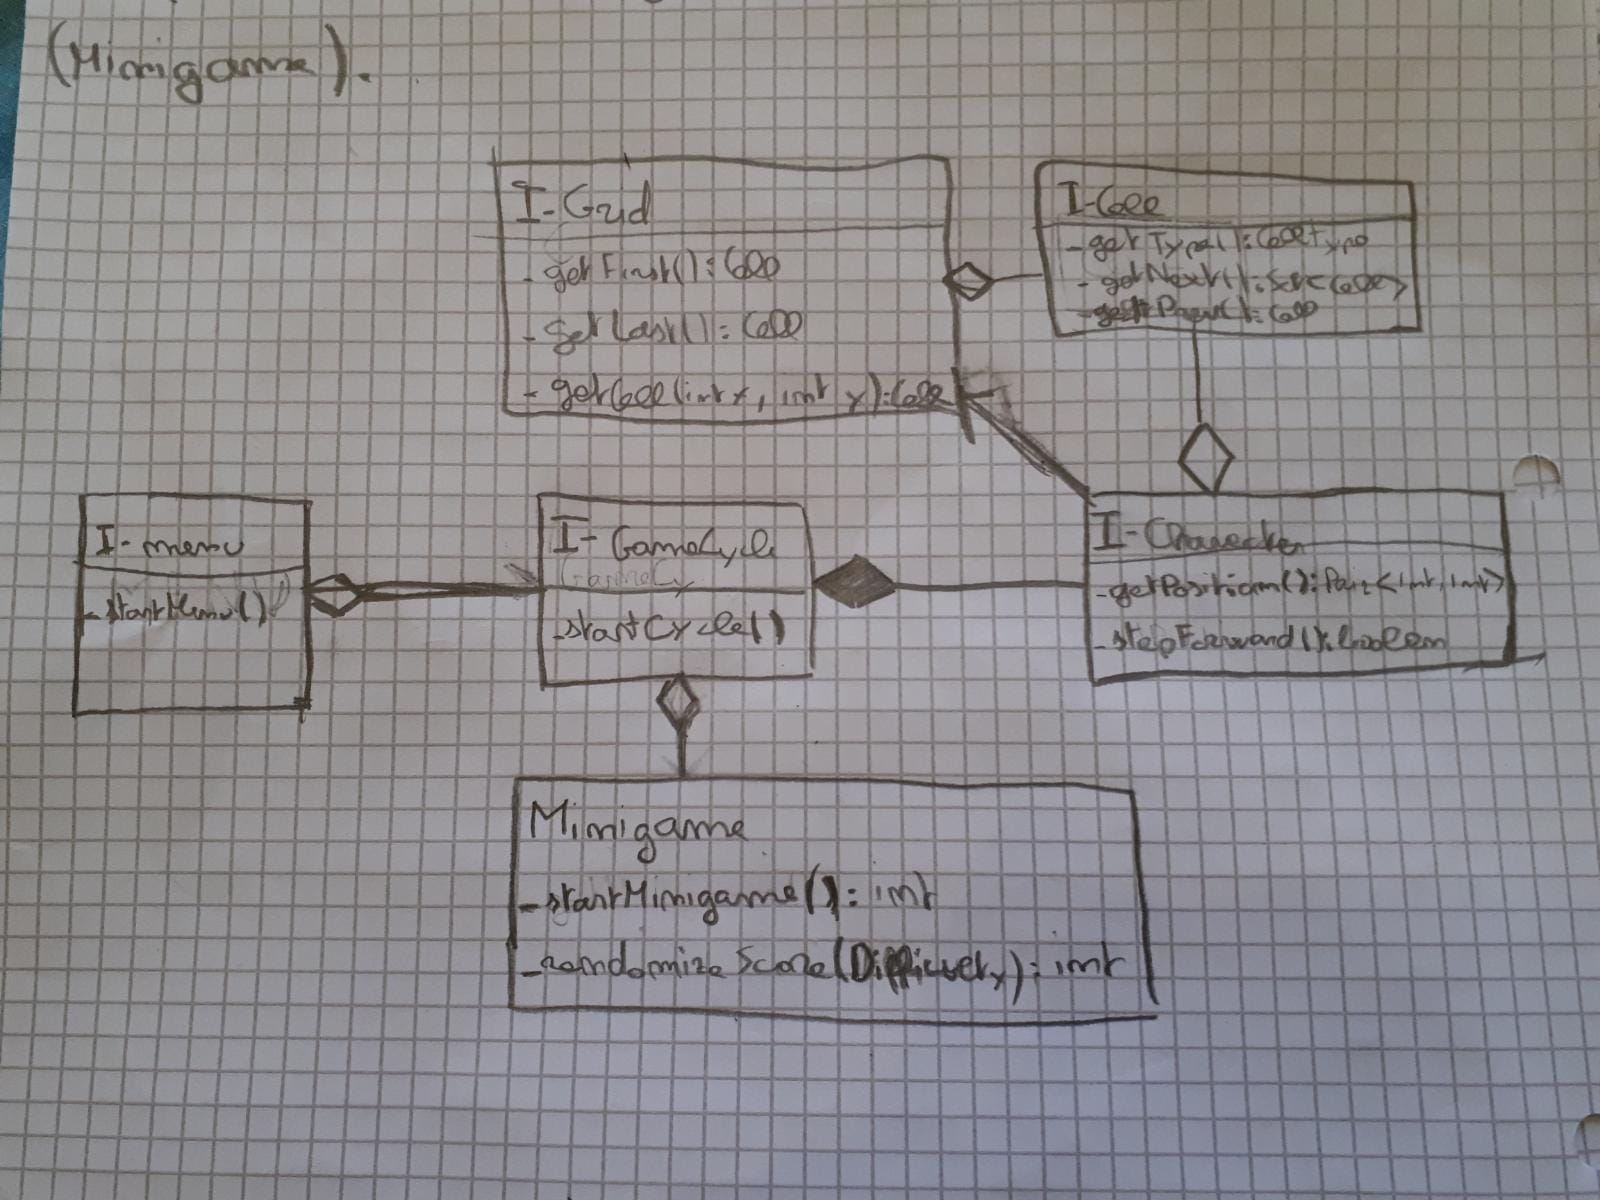
\includegraphics[width=150mm]{images/domain.jpeg}
\caption{Schema UML dell'analisi del problema, con rappresentate le entità principali ed i rapporti fra loro}
\label{img:analysis}
\end{figure}

\chapter{Design}

\section{Architettura}

L'architettura del software segue il pattern architetturale MVC.
%
Il menu è composto da una View (MenuView), e un Controller (MenuController) che ne cattura gli eventi e ne comanda le modifiche.
%
Quando il gioco viene avviato il Controller del menu avvia il ciclo di gioco (GameCycle).
%
Il ciclo di gioco avvia un nuovo thread in background che si occupa di gestire una serie di personaggi e le varie CPU, gestire la sequenza dei turni nel gioco, e aggiornare la View della griglia (Gridview) quando necessario.
%
Il Character rappresenta un personaggio in grado di tirare il proprio dado e spostarsi all'interno della griglia (Grid).
%
La CPU si occupa invece di fare le decisioni che spetterebbero normalmente al giocatore, come scegliere il percorso da fare in un bivio.
%
Il Character tiene traccia della propria posizione tramite un riferimento alla casella (Cell) su cui si trova.
%
La casella contiene delle coordinate e il riferimento alle caselle successive e precedenti nel tabellone.
%
La griglia gestisce le caselle, e permette di ottenere la prima e l'ultima casella del percorso, o una certa casella date delle coordinate.
%
Minigame si occupa di eseuire il minigioco, o ottenere un punteggio per una CPU in base alla sua difficoltà.
%
Ogni minigioco avrà a sua volta delle ulteriori interfacce di View, Controller e Model.

\begin{figure}[!t]
\centering{}
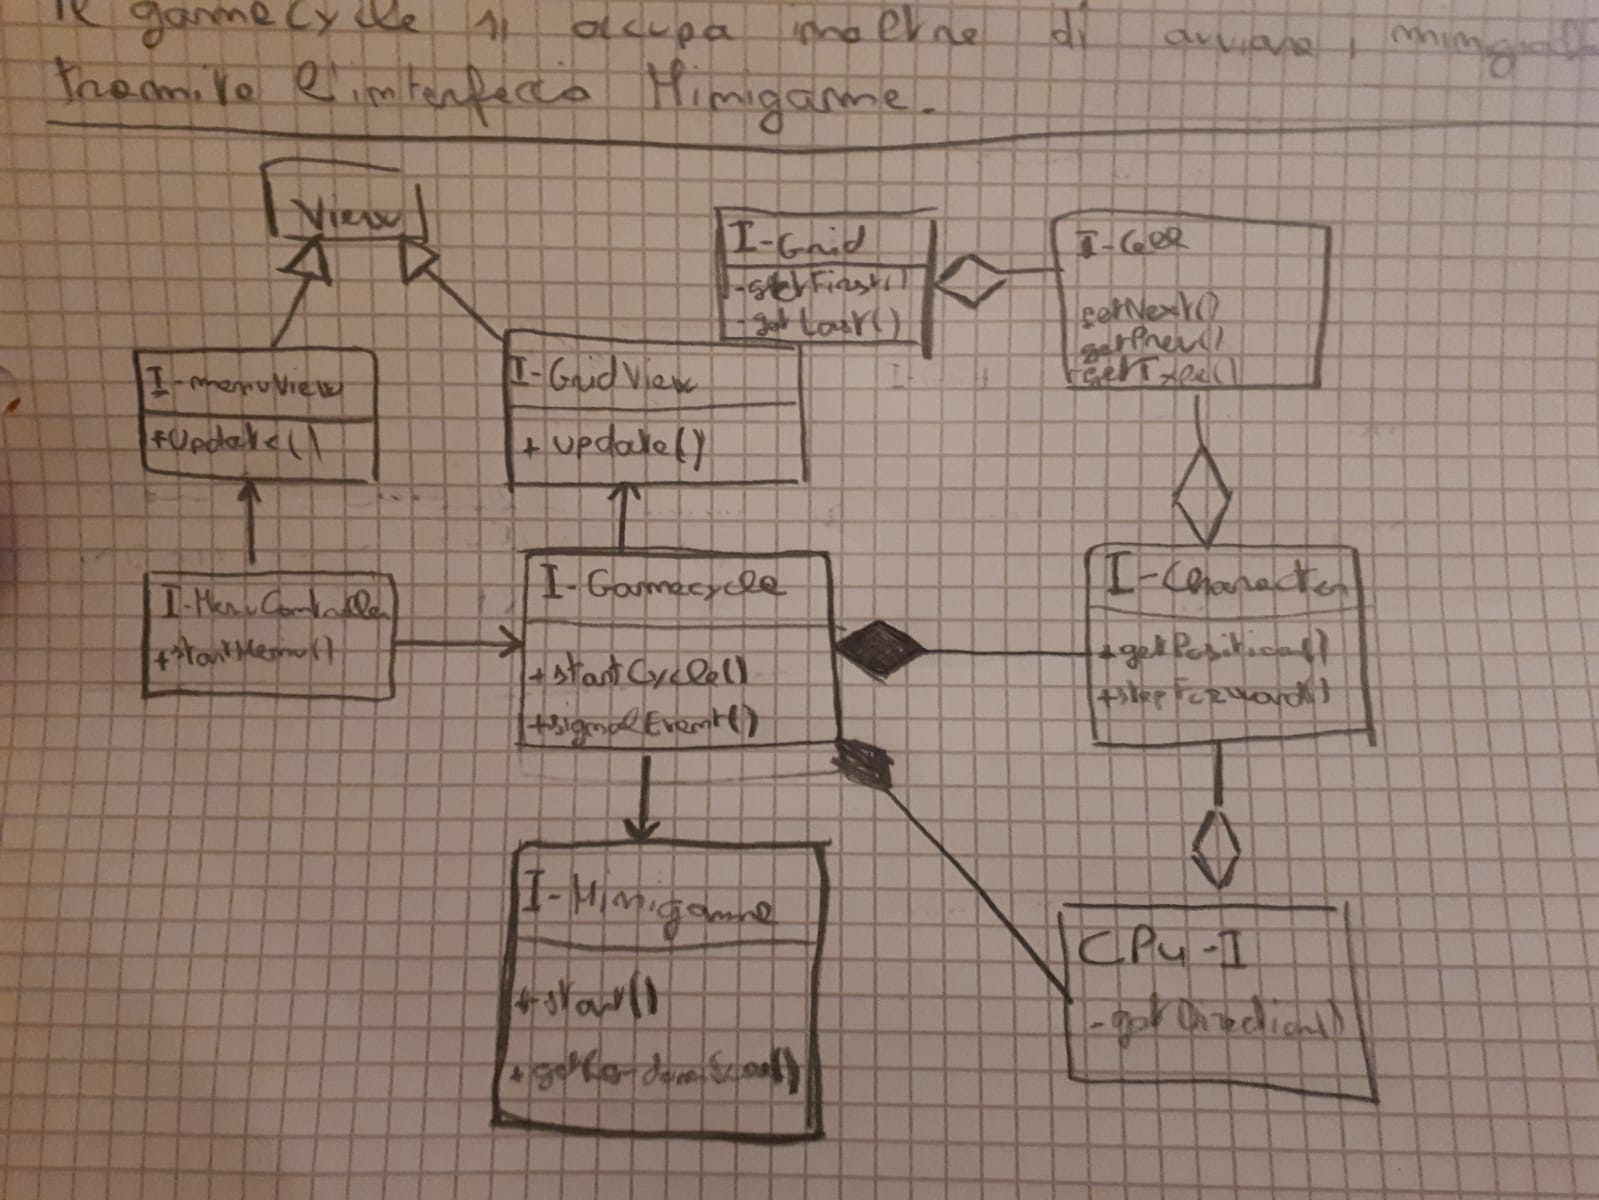
\includegraphics[width=\textwidth]{images/arch.jpeg}
\caption{Schema UML architetturale di DPG. View, GridView e MenuView sono interfacce di view, Gamecycle e Minigame sono interfacce di controller, mentre Grid, Cell e Character sono interfacce di modello.}
\label{img:goodarch}
\end{figure}

\section{Design Dettagliato}

\subsection{Design dettagliato Davide Freddi}
Design dettagliato davide freddi

\subsection{Design dettagliato Davide Picchiotti}
Design dettagliato Davide Picchiotti

\subsection{Design dettagliato Miriana Ascenzo}
Design dettagliato Miriana Ascenzo

\subsection{Design dettagliato Riccardo Squarcialupi}
Design dettagliato Riccardo Squarcialupi

\chapter{Sviluppo}
\section{Testing automatizzato}

\subsection{Davide Freddi}
\subsection{Davide Picchiotti}
\subsection{Miriana Ascenzo}
\subsection{Riccardo Squarcialupi}

\section{Metodologia di lavoro}

Descrizione separazione?

\subsection{Sezione Davide Freddi}
\subsection{Sezione Davide Picchiotti}
\subsection{Sezione Miriana Ascenzo}
\subsection{Sezione Riccardo Squarcialupi}


\section{Note di sviluppo}

\subsection{Davide Freddi}
\subsection{Davide Picchiotti}
\subsection{Miriana Ascenzo}
\subsection{Riccardo Squarcialupi}

\chapter{Commenti finali}

\section{Davide Freddi}
\section{Davide Picchiotti}
\section{Miriana Ascenzo}
\section{Riccardo Squarcialupi}

\appendix
\chapter{Guida utente}

Spiegazione comandi e utilizzo del gioco

\bibliographystyle{abbrv}
\bibliography{template}

\end{document}
